\documentclass[twoside,11pt]{article}

\usepackage{jmlr2e}
\usepackage{spverbatim}
\usepackage{amsmath}

\newcommand{\ith}{$i^{th}$ }
\newcommand{\jth}{$j^{th}$ }
\newcommand{\weight}{$w_{ji}$ }

\begin{document}

\title{Learning with Neural Nets}

\author{\name Andrew Kirby \email andy-kirby@live.com \AND
		\name Kevin Browder \email browderkevin54@gmail.com \AND
		\name Nathan Stouffer \email nathanstouffer1999@gmail.com \AND
		\name Eric Kempf \email erickempf123@gmail.com }

\maketitle

\begin{abstract}
yeet
\end{abstract}

\section{Problem Statement}

	

\subsection*{Hypothesis}
RBF is expected to preform better than MLP because it handles categorical variables where MLP does not take them into account. MLP and RBF on the raw data will out preform the clustering methods because they have more data to train on. This is especially important for the MLP with more layers because more layers require more data to adequately train.
\section{Algorithms}
\subsection{RBF Networks}
	Radial basis function networks are three layer feed forward networks consisting of an input layer, a single hidden layer, and an output layer. The activation functions in the hidden layer are of radial basis functions (RBFs)---functions whose output is determined by a $distance$ from some $center$. The non-linear nature of RBFs allow the RBF network to function as a universal approximator, approaching an arbitrary level of performance given enough centers and appropriate standard deviations $\sigma$ (CITE WU RBF.pDF). %TODO CITE THIS
	
	A popular RBF is the Gaussian, whose activation function $G$ given a data point $\vec{x}$ follows the form
	$$G(\vec{x}) = exp({\frac{-r^2}{2\sigma^2}})$$
	where $r$ is the distance between $\vec x$ and some center $\vec c$, and $\sigma^2$ is a parameter treated as variance (CITE WUUUU RBF). The RBF networks discussed in this paper will use a Gaussian activation function with distance $r$ evaluated using Euclidean distance.
	%TODO CITE THIS ANDY ^^^^^
	
	A Gaussian RBF commonly utilizes clustering to find suitable centers. Edited Nearest Neighbor, Condensed Nearest Neighbor, KMeans, and Partitioning Around the Medoids clustering methods were used to determine RBF centers. Variance $\sigma^2$ of each center $\vec c$ returned by the clustering methods may be computed in a variety of methods, including calculating the variance among the $k$ nearest neighbors of each $\vec c$. 
	
	A classification network uses an output layer with a sigmoidal neuron corresponding to each class. Predictions are evaluated as output class node with the largest value. A regression network uses a linear neuron on the output layer.for each real value to predict. Once a RBF network has been constructed using appropriate $\vec c$, $\sigma^2$, and output nodes, the output layer is trained using gradient descent (see section 2.3). 
	

\subsection{MLP Networks}
The Multilayer Perceptron (MLP) is a feed forward neural network used for classification and regression.

At its core, the MLP is composed of an input layer, hidden layers, and an output layer. Each hidden layer contains a tunable number of hidden nodes and an activation function. If the nodes in the hidden layer use a non-linear activation function, MLP becomes a universal function approximator \citep{svozil1997ffnn}.
An MLP is trained using Stochastic Gradient Descent.
To use a trained MLP, begin by using a query example as the input layer. 
% TODO discuss the prediction process

\subsection{Gradient Descent}
Recall that the performance of a Neural Network can be evaluated with an error function.
Most commonly, this error function is chosen to be the Mean Squared Error of each of the output nodes (applied appropriately to classification vs regression problems).

A given network N performs best when it's error function Err is minimized.
At first, this seems like a simple minimization problem: take the derivative of Err and find the weights that produces the smallest output in Err.
While that would be a good solution for a problem with small dimensions, the dimension of Err is same as the number of weights in the network, which can be a massive number.
This means that the classic optimization used in Calculus will be too computationally expensive to find the global minimum of Err. Thus, another technique must be used.
The technique used while training Neural Networks is Gradient Descent (GD).

Gradient Descent is an iterative process used to find a local minimum of a function. Note that only a local minimum is found, not a global minimum.
This means the performance of the Neural Network trained with GD is not necessarily optimal.
However, what is lost in performance is gained back in training time, as Gradient Descent's search for a local minimum is far more efficient than the standard search for a global minimum.

For a function $f$, GD iteratively uses the following rule for finding a local minimum:
$\Delta x_a = - \eta \dfrac{\partial f}{\partial x_a}$ where $x_a$ is value of the Err function in the $a^{th}$ dimension and $\eta$ is a tuned parameter (also called the learning rate). GD has found a local minimum once all the values of $x_a$ have converged.
Applying this to Err, gives
$$\Delta w_{ji} = - \eta \dfrac{\partial Err}{\partial w_{ji}}$$
where $w_{ji}$ is the weight from the $i^{th}$ to the $j^{th}$ node and $\eta$ is the tuned learning rate. Using the chain rule,
$\dfrac{\partial Err}{\partial w_{ji}} = \dfrac{\partial Err}{\partial net_{j}} * \dfrac{\partial net_j}{\partial w_{ji}}$. Note that $net_j = \sum w_{ji} * x_{ji}$ where $x_{ji}$ is the $i^{th}$ input to the $j^{th}$ node.

Beginning with the simpler of the partial derivatives, $\dfrac{\partial net_j}{\partial w_{ji}} = x_{ji}$.
The other partial derivative depends on two conditions: the activation function of a node and whether the node is in a hidden layer or an output layer. Let $A_j(net_j)$ denote the activation function of the \jth node, whether sigmoidal or linear. 
The value of the partial derivative also depends on the layer type of node $j$. 

Let $\delta _j^o$ denote $\dfrac{\partial Err}{\partial net_{j}}$ for the \jth node in the output layer and $\delta ^h_j$ denote $\dfrac{\partial Err}{\partial net_{j}}$ for the \jth hidden layer. 
Then, 
$$\delta _j^o = -A^\prime _j (net_j) * (d_j - o_j)$$
where $d_j$ is the target of the \jth node. And, 
$$\delta ^h_j = A^\prime _j (net_j) * \sum_{k \in ds(j)} \delta _k * w_{kj}$$ 
where $ds(j)$ returns the deltas of the nodes that the \jth node directly affects (also called the downstream nodes).

This sets up the Backpropagation Rule. This rule begins by computing each $\delta _j^o$ for each node in the output layer. Then update the weights that apply to the output layer according to 
$\Delta w_{ji} = - \eta * \delta _j^o * x_{ji}$.
Now the weights going to the output layer have been updated and the network has the necessary values of $\delta _j$ to begin a recursive call (from the last to the first hidden layer) that updates weights by the following rule
$\Delta w_{ji} = - \eta * \delta _j^h * x_{ji}$ using $\delta _j^h$ 
from above \citep{rumelhart1988learning}.

A true Gradient Descent method would average $\dfrac{\partial Err}{\partial w_{ji}}$ over the entire training set. Stochastic Gradient Descent (SGD) selects a batch of random examples from the training set and averages $\dfrac{\partial Err}{\partial w_{ji}}$ over that batch. This method, while less stable, runs much faster than true GD \citep{svozil1997ffnn}.

The final step in GD is to repeat batching and propagating the changes backwards until the weights in the network converge. Once the weights have converged, a local minimum has been found and the network is ready to use.

An option when computing GD is to include a momentum term. For a given iteration in GD, denoted 
$\dfrac{\partial Err}{\partial w_{ji}}^t$, momentum is $\alpha * \dfrac{\partial Err}{\partial w_{ji}}^{t-1}$ where $\alpha \in \mathbb{R}$, more specifically, $\alpha \in [0,0.5]$.
This gives the new update rule: 
$$\Delta w_{ji} = - \eta \dfrac{\partial Err}{\partial w_{ji}} + \alpha * \dfrac{\partial Err}{\partial w_{ji}}^{t-1}$$

A momentum term is added for two reasons. First, momentum typically causes a network to train faster because each $\Delta w_{ji}$ is a larger value \citep{rumelhart1988learning}.
The second reason is an attempt to find the best local minimum in a region. 
By moving in the direction of the previous iteration, GD may pass by a local minimum that does not offer as good of performance as another local minimum. 
However, as always, there is no free lunch and GD may well pass by a local minimum that performs better than the one it ends up finding.

\section{Experiment}

\subsection{Preprocessing Choices}
First, all the examples in the data set are randomly scrambled and then assigned to sets
for ten-fold cross validation. All categorical variables are converted to integers and the
preprocessor also generates a similarity matrix for each categorical variable that is used for
determining distances between categorical variables. All numerical variables are normalized
between 0 and 1. The data sets did not contain any missing variables.

\subsection{Evaluation Metrics}
Each algorithm's performance is evaluated using accuracy, mean square error (MSE), and mean error (ME).

For classification, the MSE metric implemented measures the squared error between the predicted and actual class distributions. This is similar in concept to a Brier score but different in computation.  Accuracy indicates how well the algorithm is classifying examples on an individual basis.

ME and MSE will be used to evaluate the regression problems. MSE takes the distance between real and predicted values and squares it. ME is computed similarly, but will not square the difference. MSE emphasizes the effect of outliers while ME captures whether the learner tends to over- or under-estimate the values in the test set. MSE and ME for regression sets are represented by a Z-Score (standard deviations from the mean) for comparability.
\subsection{Data Sets}
\subsection{Tuning}
%TODO: FIX THIS
\subsubsection{RBF}
Tuning an RBF network relies on finding the optimal centers, variances, and learning rate for a given problem. The centers were varied using the variety of clustering methods mentioned in section 2.1. Variances were found by the variance of the $k$ nearest neighbors of each center. The value of $k$ was varied during tests but ultimately set to 25. Tuning found that varying $k$ in this region did not significantly affect the performance of the RBF network as opposed to the clustering method or learning rate. Learning rate was tuned over a range of $1*10^{-4}$ to $5$. The results of the tuning process are shown in Figure 1. %TODO ADD THE FIGURE REFERENCE HERE

\begin{figure}[h]
	\centering
	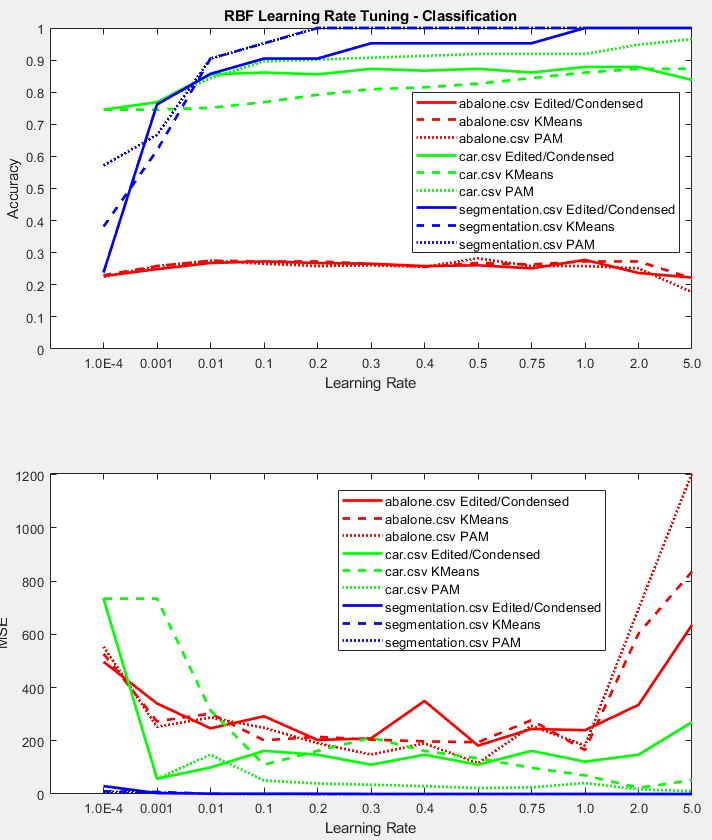
\includegraphics[height=4in]{FINAL_FIGS/RBF_LR_TUNING_CLASS.JPG}
	\caption{Results of tuning the RBF network on the classification sets. Color indicates dataset and line style indicates the clustering method used to find the centers.}
\end{figure}
\begin{figure}[h]
	\centering
	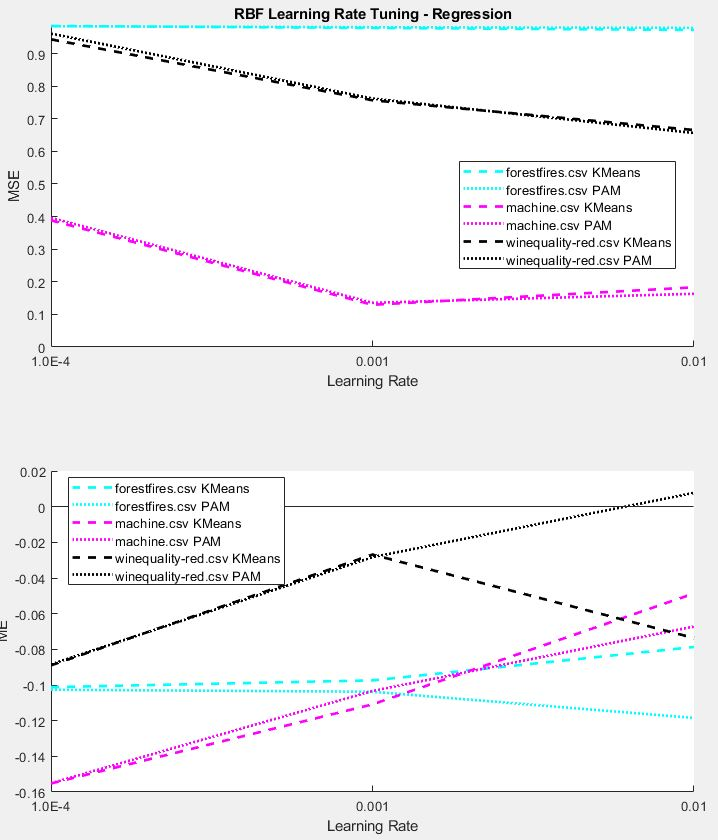
\includegraphics[height=4in]{FINAL_FIGS/RBF_LR_TUNING_REG.JPG}
	\caption{Results of tuning the RBF network on the regression sets. Color indicates dataset and line style indicates the clustering method used to find the centers.}
\end{figure}

Learning rates greater than 0.01 are not included for the regression data sets. Saturation in output layer weights caused complications in the linear output's calculations. Thus, it was determined that low learning rates were necessary to prevent network saturation in these cases.

As seen, the best clustering method used to create the RBF network varied slightly for each dataset. The classification networks performed well over a wide range of learning rates, dropping in performance only as the learning rate became too slow. The regression networks appeared to favor a midband of learning rates. The network did not learn enough at rates lower than $1*10^{-4}$ and experienced weight saturation at rates higher than $0.01$.


\subsubsection{MLP}
Tuning began with learning rate, $\eta$, which is the step size at each iteration in a neural network. The following graphs plot the MSE and accuracy for classification and MSE and ME for regression. The graphs also show performance on different numbers of hidden layers ranging from 0 to 2. Number of hidden nodes was left at 2 times the number of attributes for the tuning of all hyper parameters.
\begin{figure}[h]
	\centering
	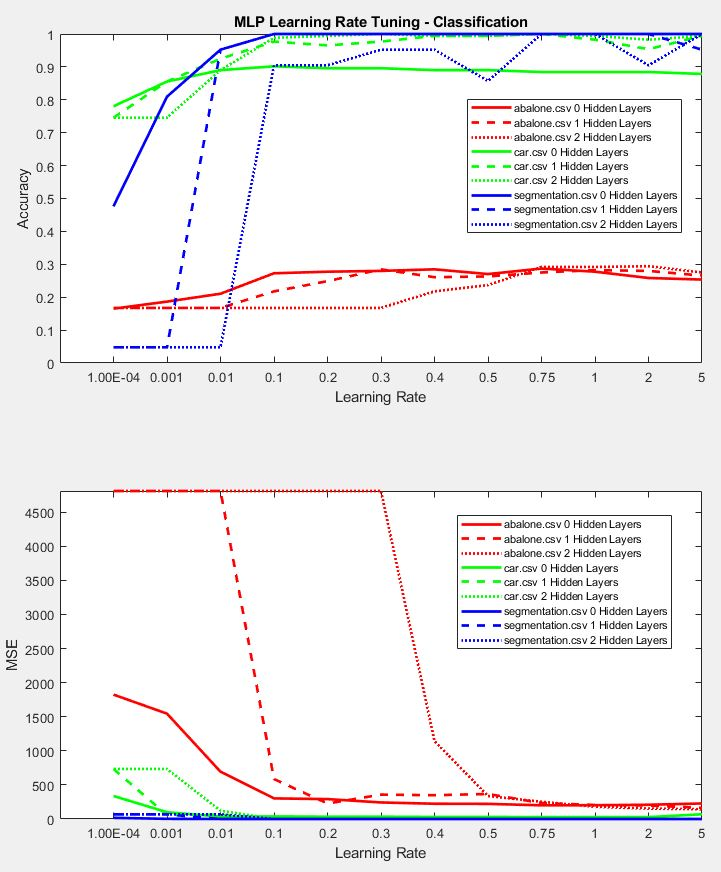
\includegraphics[height=4in]{FINAL_FIGS/MLP_LR_TUNING_CLASS.JPG}
\end{figure}
\begin{figure}[h]
	\centering
	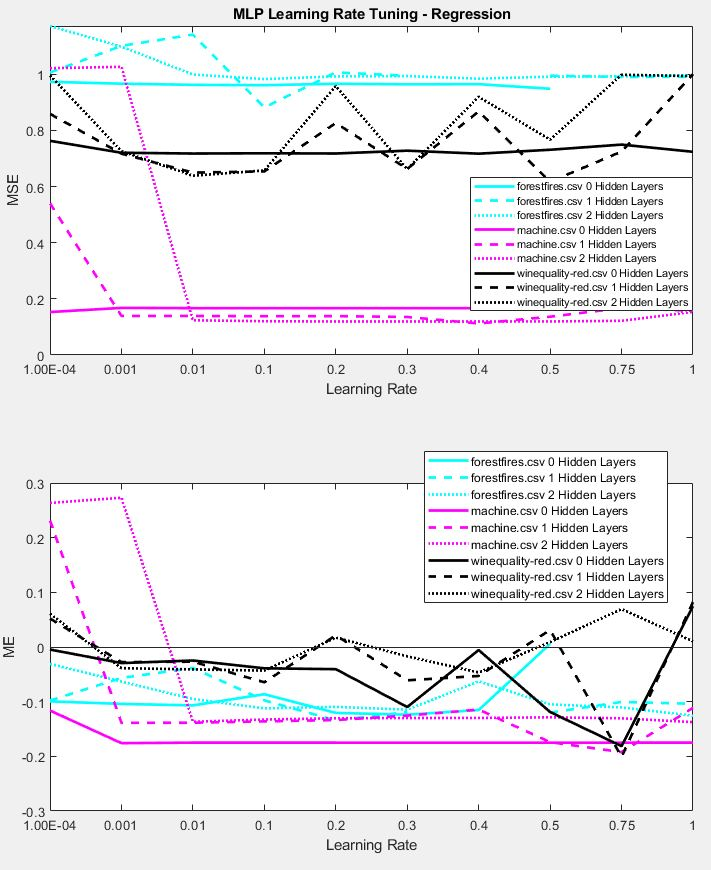
\includegraphics[height=4in]{FINAL_FIGS/MLP_LR_TUNING_REG.JPG}
\end{figure}
Beginning with the classification data sets, the initial value was set to .1. The other values tested were: .0001, .001, .01, .2, .3, .4, .5, 1, 2 and 5. Learning rates below .1 preformed the worst and rates above .1 did not see any added performance except on abalone where .2 drastically reduced the MSE which is because it was run with the same number of iterations as the other two data sets but has many more points so it requires a higher learning rate for the same performance.
On the regression data sets, the initial value and other tested values were the same as classification. Regression preformed best with a learning rate of .1 on all of the data sets. Smaller learning rates preformed significantly worse and larger learning rates have inconsistent results. \\
Another parameter must also be tuned: momentum, the rate at which a network will reach convergence. The value starts with .5 and is tuned down to .25 and 0 from there. \\
\begin{figure}[h]
	\centering
	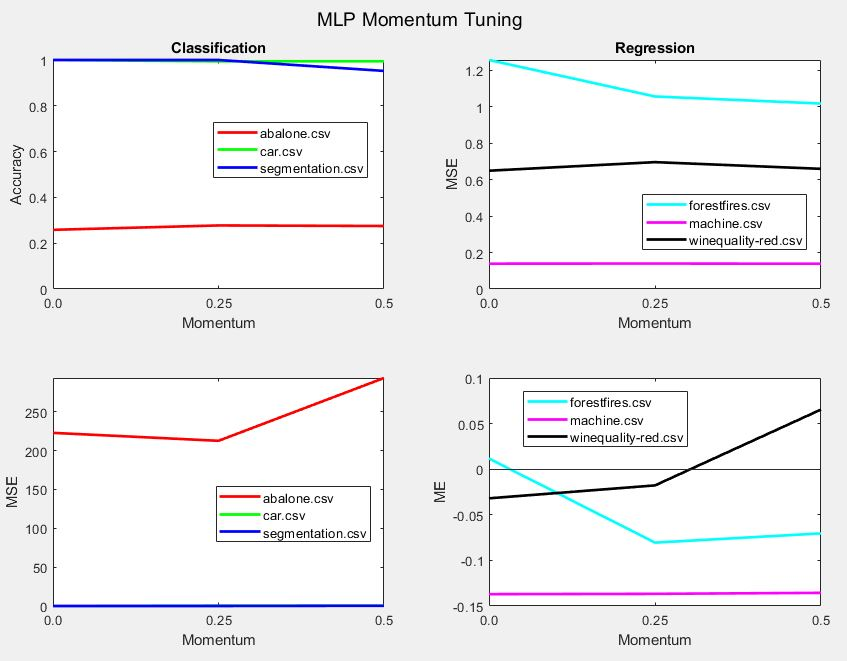
\includegraphics[height=3in]{FINAL_FIGS/MLP_MOMENTUM.JPG}
\end{figure}
On the abalone data set, MSE increased significantly when momentum was increased from .25 to .5 but accuracy had no change. The other two regression (forest fires, machine) data sets had negligible differences in the MSE and accuracy when varying momentum. The regression data sets preformed best with a momentum of .25. A larger momentum significantly increased ME on the wine quality data set while a smaller momentum significantly increased the MSE on the forest fires data set. Aside from these results, all other results were negligible from varying momentum.
\section{Results}
\begin{figure}[h]
	\centering
	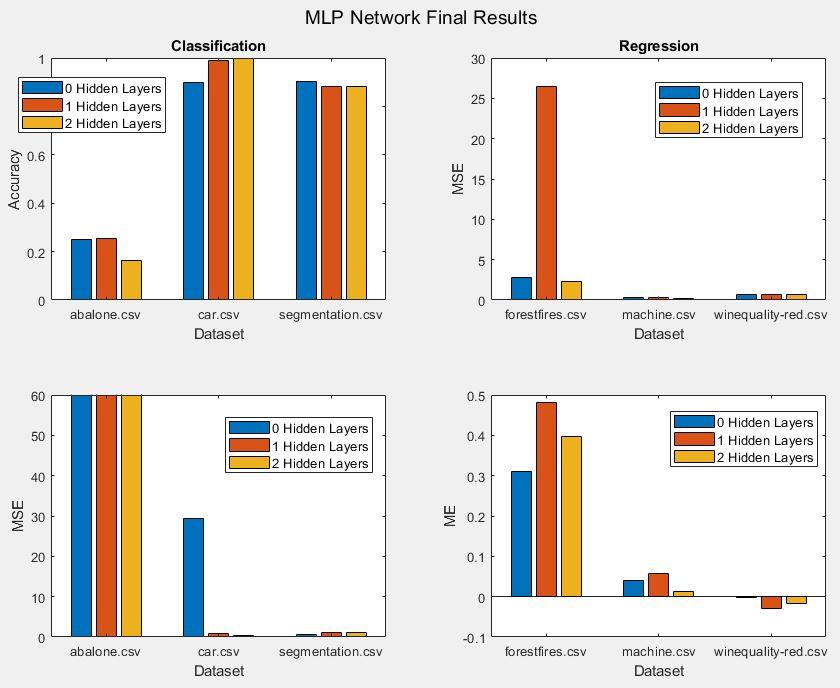
\includegraphics[height=3in]{FINAL_FIGS/MLP_FINAL.JPG}
\end{figure}
\begin{figure}[h]
	\centering
	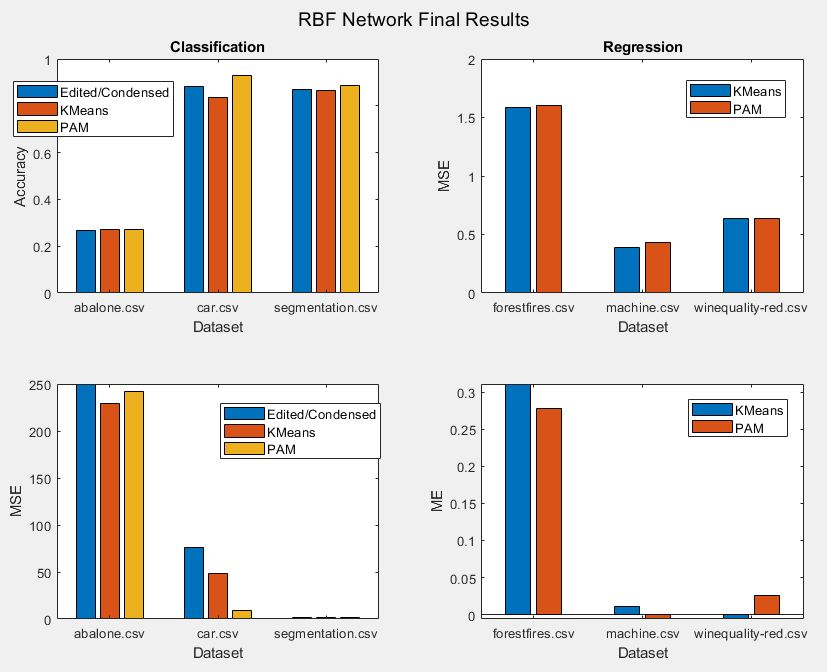
\includegraphics[height=3in]{FINAL_FIGS/RBF_FINAL.JPG}
\end{figure}
\section{Summary}


\bibliography{biblio}

\end{document}
